\documentclass[english]{article}
\usepackage[T1]{fontenc}
\usepackage[utf8]{luainputenc}
\setcounter{secnumdepth}{4}
\setcounter{tocdepth}{4}
\usepackage{color}
\usepackage{babel}
\usepackage{array}
\usepackage{graphicx}
\usepackage{setspace}
\usepackage{todonotes}
\usepackage{placeins}
\usepackage[tocentry, tablegrid,nochapter]{vhistory} 
\usepackage{catchfilebetweentags}
\usepackage{adjustbox}






\usepackage[unicode=true,
 bookmarks=true,bookmarksnumbered=true,bookmarksopen=false,
 breaklinks=false,pdfborder={0 1 1},backref=false,colorlinks=false]
 {hyperref}
\hypersetup{pdftitle={RASD},
 pdfauthor={Piazzolla Matteo Michele - Millimaggi Andrea},
 pdfsubject={RASD Documentation}}

\usepackage{fancyhdr,graphicx,lastpage}% http://ctan.org/pkg/{fancyhdr,graphicx,lastpage}
\fancypagestyle{plain}{
	\fancyhf{}% Clear header/footer
	\fancyhead[L]{Requirements Analysis and Specification Document }% Right header
	\fancyhead[R]{\emph{Issue 1}}% Right header
	\fancyfoot[L]{Piazzolla Matteo Michele - Millimaggi Andrea}% Left footer
	\fancyfoot[R]{\thepage\  / \pageref{LastPage}}% Right footer
}
\pagestyle{plain}% Set page style to plain.


\makeatletter

\providecommand{\tabularnewline}{\\}

%%%%%%%%%%%%%%%%%%%%%%%%%%%%%% Textclass specific LaTeX commands.
\newcommand{\lyxrightaddress}[1]{
\par {\raggedleft \begin{tabular}{l}\ignorespaces
#1
\end{tabular}
\vspace{1.4em}
\par}
}

%%%%%%%%%%%%%%%%%%%%%%%%%%%% contatore requirement
\newcounter{requirement}
\setcounter {requirement} {0} 

\newcommand{\reqcounter}{
\stepcounter{requirement}
\item \textbf{[R-\arabic{requirement}]}
}


%%%%%%%%%%%%%%%%%%%%%%%%%%%% comando per generare i goal
\def\CatchFBT@sanitize{%
	\@sanitize
	\@makeother\{%
	\@makeother\}%
	\ifluatex\else
	\endlinechar=`\^^J%
	\fi
}% 

\newcommand{\goal}[1]{
{[}G#1{]}\ExecuteMetaData[goals]{#1}
}

%%%%%%%%%%%%%%%%%%%%%%%%%%%% comando per la tabella degli use case
\newcommand{\usecase}[8]{
	\begin{center}
	\begin{adjustbox}{max width=\textwidth}	
		\begin{tabular}{|l|>{\raggedright}p{15cm}|}
			\hline 
			Use Case Name & #1\tabularnewline
			\hline 
			\hline 
			Actors & #2\tabularnewline
			\hline 
			Goals & #3\tabularnewline
			\hline 
			Preconditions & #4\tabularnewline
			\hline 
			Postconditions & #5\tabularnewline
			\hline 
			Normal Flow & #6
			\tabularnewline
			\hline
			Alternative Flows & #7
			\tabularnewline
			\hline
			Exceptions & #8
			\tabularnewline
			\hline 
		\end{tabular}
		\end{adjustbox}	
	\par\end{center}
	}

%%%%%%%%%%%%%%%%%%%%%%%%%%%% tabella dei vari issue 
\newcommand{\revisionhistory}{

	\begingroup
	\fontsize{15pt}{12pt}\selectfont
	\textbf{Revision History}
	\endgroup

	\begin{versionhistory}
		\vhEntry{1.0}{13/11/16}{Piazzolla  Millimaggi }{First document issue}
		\vhEntry{ }{ }{ }{ }
		\vhEntry{ }{ }{ }{ }
	\end{versionhistory}}

\makeatother

%%%%%%%%%%%%%%%%%%%%%%%%%%%% inizio documento
\begin{document}

\title{
\includegraphics[scale=0.4]{img/polimi}\\
Computer Science and Engineering}

\begin{doublespace}

\author{A.A. 2016/2017\\
Software Engineering 2 Project: \\
\\
{\LARGE{}``PowerEnJoy''}\textbf{}\\
\\
\textbf{R}equirements \textbf{A}nalysis and \textbf{S}pecification
\textbf{D}ocument\\
}
\end{doublespace}

\maketitle
\thispagestyle{empty}
\lyxrightaddress{Prof.Luca Mottola\\
\\
Matteo Michele Piazzolla Matr. 878554\\
Andrea Millimaggi Matr. 876062}

%%%%%%%%%%%%%%%%%%%%%%%%%%%%
\newpage{}

\listoftodos

%%%%%%%%%%%%%%%%%%%%%%%%%%%%
\newpage{}

\revisionhistory

%%%%%%%%%%%%%%%%%%%%%%%%%%%%
\newpage{}

\tableofcontents{}

%%%%%%%%%%%%%%%%%%%%%%%%%%%%
\newpage

\listoffigures

%%%%%%%%%%%%%%%%%%%%%%%%%%%%
\newpage{}

\section{INTRODUCTION}
\subsection{Purpose and Scope}
\subsubsection{Purpose}
The purpose of this document is to provide an estimation of the cost and the size of the project. This knowledge is needed to organize the resources needed in the development of the system and to properly schedule the activities of the project.\newline
To reach this purpose, two models will be used:
\begin{itemize}
\item \textbf{Function Point:} This approach is used to estimate the size of the project in LOC.
\item \textbf{COCOMO:} This model is used to estimate the effort required by the project in PM.
\end{itemize}

\subsubsection{Scope}
PowerEnJoy is a digital system for the management of a car-sharing service that only employs electric cars. In particular the aim is to develop a mobile application that allows the user to pick up and use electric cars in the areas reached by the service.

\subsection{List of Definitions and Abbreviations} 
\subsubsection{Acronyms}
\begin{itemize}
\item RASD: Requirement Analysis and Specification Document.
\item DD: Design Document.
\item DBMS: Database Management System.
\item DB: Database.

\item GPS: Global Positioning System

\end{itemize}
\subsubsection{Definitions}

\subsubsection{Abbreviations}
\begin{itemize}
	\item  FP: Function Points.
	\item  ILF: Internal logic file
	\item  ELF: External logic file.
	\item  EI: External Input.
	\item  EO: External Output.
	\item  EQ: External Inquiries.
	\item PH: Person Hours.
	\item LOC: Lines Of Code.
\end{itemize}



\subsection{List of Reference Documents}
\begin{itemize}
	\item PowerEnJoy RASD.	
	\item PowerEnJoy DD.
	\textbf{NOTE:} The reader must refer to the version 1.1 of the DD.
	\item COCOMO II Model Definition Manual 
\end{itemize}



\section{Overall Description}



\subsection{Product perspective}\todo[inline]{(further details on the shared phenomena and a domain model{-->}class diagrams and statecharts)}
The system that we are going to develop is made of several parts. 
\begin{itemize}
	\item A Mobile Application usable from every Tablet or Smartphone that has access to an internet connection. The application will be available on Android and iOS. 
	\item A Website where a user can find information about the service.
	\item A Server backend to manage the service.
\end{itemize}

\subsubsection{System interfaces}
The system will depend on a device installed onboard every 'PowerEnJoy car. That onboad device will communicate with the user and via internet to the server.

\subsubsection{User interfaces}
The available interfaces will be:
\begin{itemize}
	\item the mobile application
	\item the website
\end{itemize}
The website will be implemented with a responsive design to adapt to all most common screen aspect and resolution with clear and minimal UI to favorite accessibility.
The mobilie application will be graphically similar to the website with a few views.
The use of the website or the mobile application won't be necessary during driving. 

\subsubsection{Hardware interfaces}
The main hardware interaction concerns the geolocalization feature, and in particular the GPS hardware on the smartphone device.
The application need an internet connection so a smart device with a 3G or LTE connectivity is required.

\subsubsection{Software interfaces}
To provide the best use of the service through the website an HTML5 compliant browser is required and an up to-to-date version of Android or iOS operating system for the mobile application.





\subsection{User characteristics}
Everyone who has a car license will be able to register to the car-sharing service and drive one of the electric car available.
Because of the variety of people that will use the service, the mobile application must be simple and user-friendly, so that anyone can use it even if it has a little knowledge about the use of a mobile device.

\subsection{Constraints}



\subsection{Assumptions}
\todo{Da completare!}
\begin{enumerate}
	\item Cars can be parked in every area of the city where the parking is allowed, either it is free or chargeable. The company 		                    takes care of the payment for chargeable parkings. 
	\item Every car can be uniquely recognized by his plate number.
	\item The position of the users are well-known thanks to GPS.
	\item The user is the one and only who drives the cars he reserves.
	\item Any user who reserves a car has enough money on his credit card to pay the travel.
	\item Every car is periodically checked to ensure proper operation.
	\item The travel of a driver is considered finished when the the engine is off and after a minute from the moment in which he closes the car doors.
\end{enumerate}

\subsection{Regulatory policies}
It’s user responsibility to ensure that the use of the system complies with the local laws and policies. If the user register to the service must allow for the permission to acquire, store and process personal data and web cookies. The system must offer to the user the possibility to delete the account and all the personal data.


\subsubsection{Possible Future Implementations}
Depending on the success that the developed system will have, it will be possible to extend the car-sharing to Scooters and Mini-Cars, in order to reach also younger customers.
\\ \noindent 
Another possibility for the future is to allow users to get in touch with strangers and pick them up in the middle of the travel.
\todo {da sistemare la seconda frase}
\\Another future improvement could be the possibility for the users share a trip with strangers and split the charge as other services like BlaBlaCar. 
\pagebreak{}

\subsection{Product requirements}
\subsubsection{Functional Requirements}

\begin{itemize}
	\item User registration
	\item Login
	\item Check for cars availability using user's position
	\item Check for cars availability using address
	\item Reserve a car
	\item Cancel a reservation
	\item Check the amount paid for a travel
	\item Check the log of reservations done
	\item View the details of cars available (level of the charge)
	
	
\end{itemize}




\pagebreak
\section{Specific Requirements}


\subsection{Functional Requirement}

With these requirements, we define features and functions with which
the user will interact directly.



\subsubsection{\goal{1}}
\begin{itemize}
	\reqcounter The system shall allow registration only if the patent license number is provided.
	\reqcounter The system shall provide a home page in which a guest user must be
	able to know what the service is. 
	\reqcounter The system shall demand the User to read and accept all term of use of the service.
	\reqcounter The system shall provide a form in which a Guest can insert his personal data for the registration to the service.
	\reqcounter The system shall provide a form in which a Guest can insert his payment information.
	
	
\end{itemize}

\subsubsection{\goal{2}}
\begin{itemize}
	\reqcounter The system shall show a sign-up page with a login form and a logout button if the User is already logged in.
	\reqcounter The system shall validate any input in both client and server side.
	\reqcounter The system shall prevent anyone from logging more than once at a time.
	\reqcounter The system shall show and error message in case of wrong credential.
	\reqcounter The system shall provide a password recovery procedure.
	\reqcounter The system shall prevent bruteforce attack limiting the number of try per IP address.
	\reqcounter The system shall redirect the User to the homepage as a guest after the logout.
\end{itemize}



\subsubsection{\goal{3}}
\begin{itemize}
	\reqcounter The system shall show a an account page with all the information that the User sent during 
	account registration.
	\reqcounter The system shall ask for the password before saving the edited details.
	\reqcounter The system shall send and email to notify the changes.
\end{itemize}



\subsubsection{\goal{4}}
\begin{itemize}
	\reqcounter The system shall show on a web page or a view in the application the position of the available car.
	\reqcounter The system shall allow the User to set a search radius.
	\reqcounter The system shall ask the User for the GPS position or to provide an address.
\end{itemize}


\subsubsection{\goal{5}}
\begin{itemize}
	\reqcounter The system shall not allow the User to request multiple cars at the same time.
	\reqcounter The system shall check if the payment information are valid and show an error if not.
	\reqcounter The system shall automatically cancel a car reservation and make the car available again if the User don't unlock the car in one hour and charge with a 1 euro fee.
	\reqcounter The system shall check for the User position and if the distance from the car is less than 50 meters
	allow to unlock the car.
	\reqcounter The system shall allow the user to be informed about the autonomy,the battery level, the model, the engine size of 		the available cars 
\end{itemize}

\subsubsection{\goal{6}}
\begin{itemize}
	\reqcounter The system shall inform the User if she is driving outside the city area.
	\reqcounter In case of driving outside the city area the system shall charge a 100\%  more of the current charge.
	\end{itemize}



\subsubsection{\goal{7}}

\begin{itemize}
	\reqcounter The system shall inform the User of the amount that will be charged.
	\reqcounter The system shall inform the User of the position of charging stations nearby the current car position.
	\reqcounter The system shall show on a map the special parking area and the safe area nerby the current car position.
           \reqcounter The system shall inform the user if she's driving more than 3 km far from the nearest power grid station
 
\end{itemize}


\subsubsection{\goal{8}}
\begin{itemize}
	\reqcounter The system shall detect the number of passengers on the car
	\reqcounter The system shall apply a discount of 10\% on the last ride if it detects the presence of two other passengers on the car in addition to the user.
	\reqcounter The system shall check the level of the battery when a car is left.
	\reqcounter The system shall apply a discount 	of 20\% on the last ride if it detects that the car was left with no more than 50\% of the battery empty.
	\reqcounter The system shall check if the user plugges the car into the power grid when he left the car in a special parking area.
	\reqcounter The system shall apply a discount 	of 20\% on the last ride if it detects that the user takes care of plugging the car into the power grid when he leaves the car in a special parking area. 
	\reqcounter The system shall calculate the distance from the parking position to the nearest power grid station and if that distance is more than 3 km, shall charge the 30\% on the last ride. 
		
\end{itemize}


\subsubsection{\goal{9}}
\begin{itemize}
	\reqcounter The system shall detect the car turning off and the closure of the doors and stop charging the user after this two actions are accomplished
	
\end{itemize}


\subsubsection{\goal{10}}
\begin{itemize}
	\reqcounter The system shall detect that the car is plugged into the power grid and start charging the battery

\end{itemize}

\subsection{Non-Functional Requirement}



\begin{itemize}
	\item PowerEnJoy has to be available 24h/7d.
	\item Both mobile application and website must be reactive and usable.
	
\subsubsection{Reliability}%affidabilità

The service has to guarantee an 24h/7d availability. Components of the project code will be tested after the implementation phase to ensure that they are functional. 
All the critical software bugs found must be patched in at least 48h.
If a Back-End API change occurs, it must be guaranteed a support for clients that implement older API.
All the system data must be constantly backed up to assure the data recovery in case of fault.

\subsubsection{Security}

The system must ensure that all data is protected from unauthorized
access. Password should be saved on a DB hashed and salted.
Every input from the user and every request must be sanitized 
\iffalse
It must support communication protocols used by web applications and
devices on or within the network edge. These include network transport
protocols such as HTTP and SSL/TLS, plus proxy support.
\fi

\subsubsection{Usability}
\begin{itemize}
	\item The User must be able to use the system with mouse, keyboard and touchscreen.
	\item The User must be able to choose from several language.
	\item At the first login the system must provide a simple and skippable 3-views guided tutorial of the service.
\end{itemize}
\end{itemize}

\begin{figure}[h]
	\centering
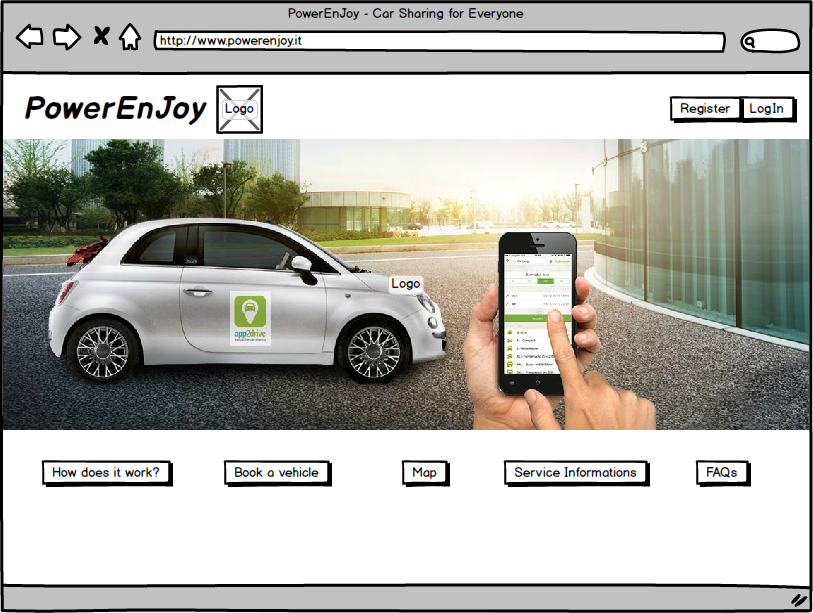
\includegraphics[scale=0.4]{img/webhome}
	\caption{PowerEnJoy website homepage}
\end{figure}
\FloatBarrier

\begin{figure}[h]
	\centering
	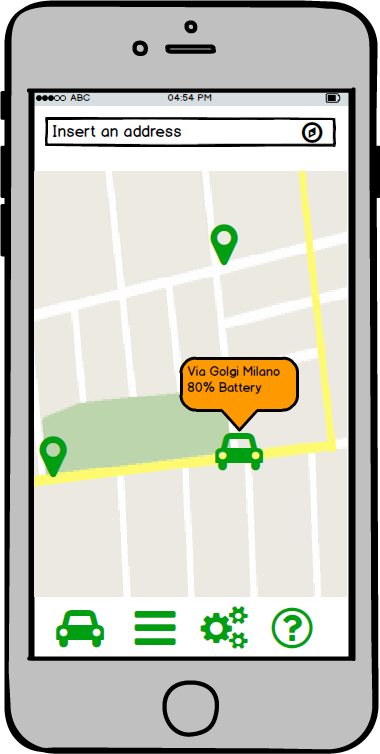
\includegraphics[scale=0.4]{img/appmap}
	\caption{PowerEnJoy Mobile Application map view}
\end{figure}
\FloatBarrier




\pagebreak
\subsection{Use Case}

\subsubsection{User Registration}

	% example \usecase{name}{actor}{goal}{precondition}{post condition}{flow}{exception}


	
	
	
	\usecase{User Registration}
				{Guest}
				{\goal{1}}
				{Guest hasn't registered to the webapp yet.}
				{Guest is signed-up and promoted to ``PowerEnJoy'' User.}
				{
					\begin{enumerate}
						\item Guest accesses to the webapp or the mobile application
						\item Guest clicks on ``Sign Up'' button
						\item Guest fill Sign-up form fields, entering\\
						-Name\\
						-Surname\\
						-Email address\\
						-Password\\
						-Telephone Number\\
						-Driving License number
						\item Guest accepts the term of use
						\item Guest clicks on ``Confirm'' button\end{enumerate}
				}
				{-}
				{
				\begin{enumerate}
					\item At least one field is empty
					\item At least one field is invalid
					\item Entered email is already associated to another account\end{enumerate}
				}
	



\pagebreak
\subsubsection{User Login}\label{login}

\usecase{User Login}
{User}
{\goal{2}}
{User has signed-up as PowerEnJoy User.}
{User is redirected to personal area.}
{
	\begin{enumerate}
		\item User accesses to the webapp or the mobile application
		\item User clicks on ``Log-in' button
		\item User fills username and password fields of Log-in form
		\item User clicks on ``Submit'' button
	\end{enumerate}
}
{-}
{
	\begin{enumerate}
		\item Invalid username and/or password
		\item At least one field is empty
	\end{enumerate}
}

\begin{figure}[h]

	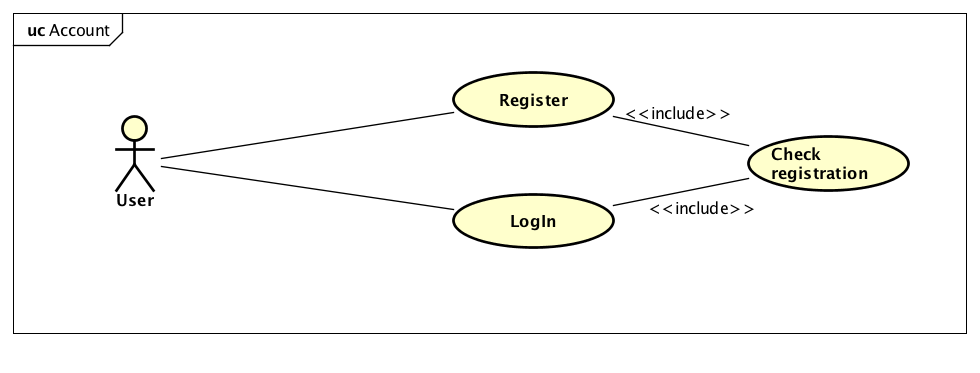
\includegraphics[width=380px]{img/usecase_login_registration}
	\caption{Use Case Login and Registration procedure. Refer to Goal 1 and 2}
\end{figure}
\pagebreak


\subsubsection{Modification of personal details and payment information}
\usecase{Modification of personal details and payment information}
{User}
{\goal{3}}
{User is logged in}
{User is redirected to the modifications area where he can modify his personal information}
{
\begin{enumerate}
	\item User clicks on ``Personal Details' button in his personal area. A page with the personal data of the user is shown'
	\item User clicks on ``Modify Data'' button. A form for modifications is shown
	\item User fills fields he wants to modify
	\item User clicks on ``Confirm'' button
	\item User is redirected to his personal area
\end{enumerate}
}
{-}
{-}
\pagebreak


\subsubsection{Search of available cars}\label{search}
\usecase{Search of available cars}
{User}
{\goal{4}}
{User is logged in}
{User is redirected to a page with the list of the available cars}
{
\begin{enumerate}
	\item User clicks on ``Search a car'' button in his personal area. A form is shown
	\item User select a distance from the ``Distance from your position'' field
	\item User clicks on ``Confirm'' button
	\item User is redirected to a page showing the available cars
\end{enumerate}
}
{
\begin{itemize}
\item Different flow from step 2:
	\begin{enumerate}
	\item[2] User write an address in the ``Address'' field 
	\item[3] User clicks on ``Confirm'' button
	\item[4] User is redirected to a page showing the available cars
 
\end{enumerate}

\end{itemize}


}
{
\begin{enumerate}
\item There aren't available cars within the distance set 
\item There aren't available cars near the address set
\end{enumerate}
}
\pagebreak

\subsubsection{Search of resources on a map}\label{search2}
\usecase{Search of resources on a map}
{User}
{\goal{5}}
{User is logged in}
{User is redirected to a page with a map where resources (available cars, safe areas, special parking areas)  are shown}
{
\begin{enumerate}
	\item User clicks on ``Search resources on the map'' button. A form is shown
	\item User select a distance from the ``Distance from your position'' field
	\item User clicks on ``Confirm'' button
	\item User is redirected to a page showing the resources on a map.
\end{enumerate}
}
{
\begin{itemize}
\item Different flow from step 2:
	\begin{enumerate}
	\item[2] User write an address in the ``Address'' field 
	\item[3] User clicks on ``Confirm'' button	
	\item[4] User is redirected to a page showing the resources on a map.
 
\end{enumerate}

\end{itemize}


}
{
\begin{enumerate}
\item There aren't available cars within the distance set 
\item There aren't available cars near the address set
\end{enumerate}

}
\pagebreak


\subsubsection{Request and Unlock}\label{request}
\usecase{Request and Unlock}
{User}
{\goal{6} \newline \goal{10} \newline \goal{11}}
{User is logged in and has searched a car (\ref{search}, \ref{search2}}
{The car requested is reserved for the user}
{
\begin{enumerate}
	\item User selects a car from the list. 
	\item A page with information about the car (battery level, model, engine size) is shown
	\item User clicks the ``Request'' Button''
	\item The car is reserved for the user
	\item User reaches the car and is less than 3 meters far from the car
	\item User unlocks the car clicking on the ``Unlock'' button in the application

\end{enumerate}
}
{
\begin{itemize}
\item Steps 1 is different:
	\begin{enumerate}
	\item[1] User select a car on the map.   
	\end{enumerate}
\item Different flow from step 5:
	\begin{enumerate}
	\item[5] An hour passes without the User unlocking the car
	\item[6]The system charges the User with an extra fee of 1 euro
	\item [7]The system cancels the request and makes the requested car available again
	\end{enumerate}
\end{itemize}


}
{
\begin{enumerate}
\item The car selected has been requested by another user before the User has clicked on the ``Request'' button.
\end{enumerate}
}
\pagebreak


\subsubsection{Driving}
\usecase{Driving}
{Driver}
{\goal{7} \newline \goal{9} \newline \goal{12} \newline \goal{13}}
{Driver is logged in and has searched, requested and unlocked a car}
{-}
{
\begin{enumerate}
\item Driver enters the car, eventually also other passengers enter the car
\item Driver starts driving
\item The system detects the number of passengers
\item The screen shows a map with the position of the car, the safe areas and special parking areas near the car position
\item The screen shows the money to be charged up to the current moment
\item The system charges the standard fee every minute.
\item Driver parks and exit the car and, if any, the other passengers exit the car
\item The system locks the car
\item The system detects the level of the battery
\item The system detects if the car has been plugged in a power grid
\item The system detects the position of the left car
\item The system applies a discount on the ride of the:
	\begin{itemize}
	\item 10\%, if it has detected the presence of at least two other passengers in addition to the driver during the travel
	\item 20\%, if it has detected that the car was left with no more than the 50\% of the battery empty
	
	\end{itemize}
\item The system charges the 30\% more on the last ride if it detects that the car has been left more than 3 km far
	from the nearest power grid station
	\end{enumerate}
\item The system takes the money from the User, using his selected payment method
}
{
	\begin{itemize}
	\item Before the last step, the system detects the presence of at least two other passengers in addition to the driver during the 		         travel and so applies a 10\% discount on the ride
	\item Before the last step, the system detects that the car was left with no more than the 50\% of the battery empty and so 			         applies a 10\% discount on the ride
	\item At step 7 the Driver parks the car in a special parking area and plugs the car into the power grid. Before the last step the 
	         the system detects that the car has been plugged into the power grid and so applies a 20\% discount on the ride
	\item While driving the Driver exits the city area. So:
		\begin{enumerate}
		\item An acoustic signal is emitted by the screen
		\item A message is shown on the screen, warning the Driver that he has exited the city area
		\item The system charges the 100\% more than the standard fee every minute until the driver re-enters in the city area
		\end{enumerate} 
	\end{itemize}

}
{-}
\todo{C'è da fare chiarezza su city area/ safe area}





\FloatBarrier




\section{Activity Diagram}
\subsection{PowerEnJoy Trip}
\begin{figure}[h]
	\centering
	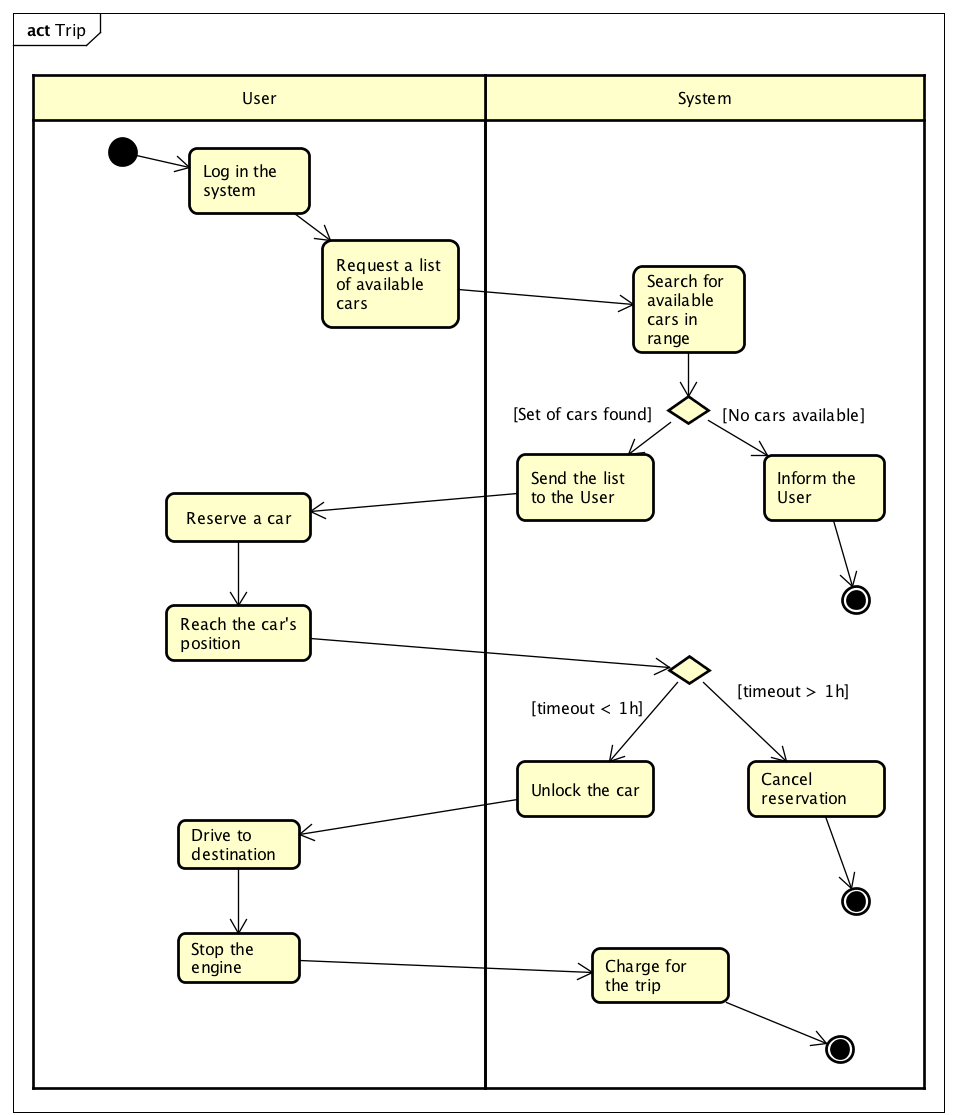
\includegraphics[width=345px]{img/activity_trip}
	\caption{PowerEnJoy normal flow}
\end{figure}
\FloatBarrier

\pagebreak
\section{Class Diagram}
\subsubsection{PowerEnJoy server}
\begin{figure}[h]
	\centering
	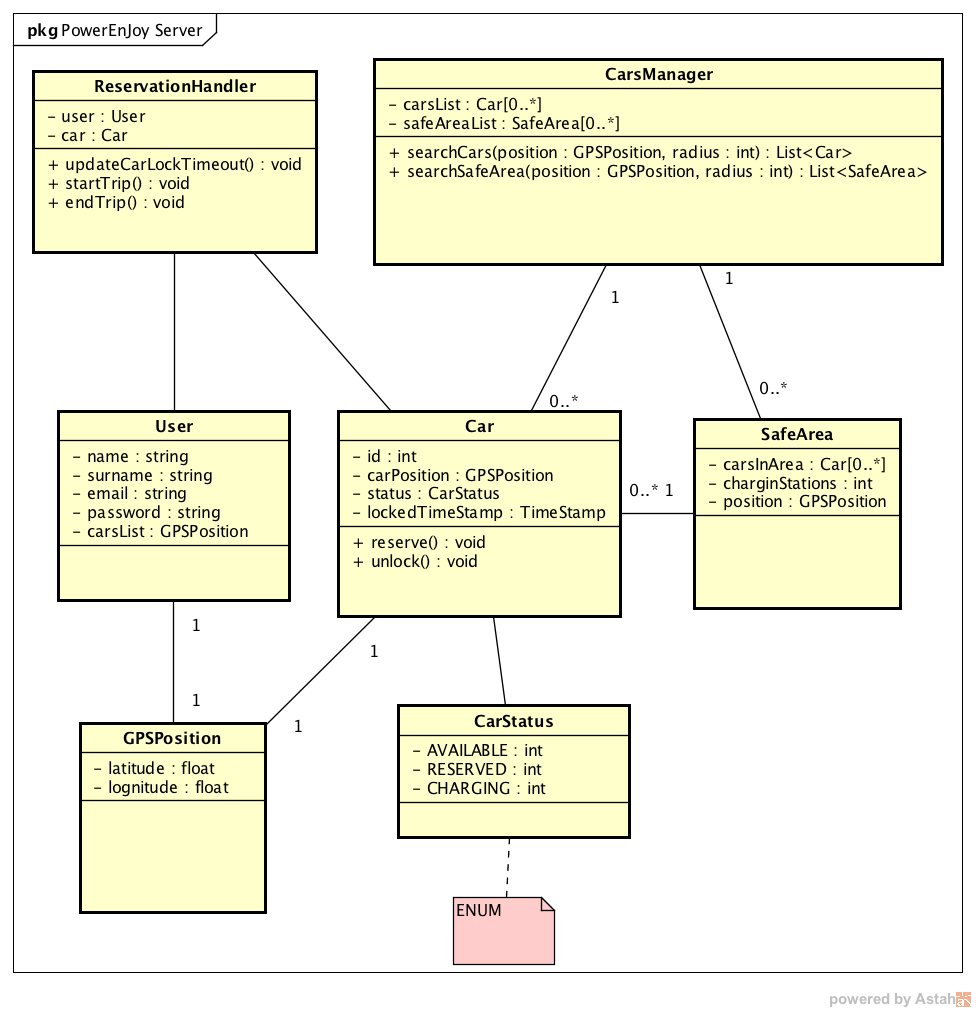
\includegraphics[width=380px]{img/classdiagram_server}
	\caption{PowerEnJoy Server Class Diagram}
\end{figure}
\FloatBarrier


\pagebreak


\section{ORE}
23/10/16 
Matteo 3h 
Andrea XX\\
24/10/16 
Matteo 3h\\
25/10/16 
Matteo 1h\\
01/11/16
Matteo 1h\\
02/11/16
Matteo 3h\\



\end{document}
